% !TEX TS-program = pdflatex
% !TEX encoding = UTF-8 Unicode

\documentclass[11pt]{article} % use larger type; default would be 10pt

\usepackage[utf8]{inputenc} % set input encoding (not needed with XeLaTeX)

%%% Examples of Article customizations
% These packages are optional, depending whether you want the features they provide.
% See the LaTeX Companion or other references for full information.

%%% PAGE DIMENSIONS
\usepackage{geometry} % to change the page dimensions
\geometry{a4paper} % or letterpaper (US) or a5paper or....
% \geometry{margin=2in} % for example, change the margins to 2 inches all round
% \geometry{landscape} % set up the page for landscape
%   read geometry.pdf for detailed page layout information

\usepackage{graphicx} % support the \includegraphics command and options

% \usepackage[parfill]{parskip} % Activate to begin paragraphs with an empty line rather than an indent

%%% PACKAGES
\usepackage{booktabs} % for much better looking tables
\usepackage{array} % for better arrays (eg matrices) in maths
\usepackage{paralist} % very flexible & customisable lists (eg. enumerate/itemize, etc.)
\usepackage{verbatim} % adds environment for commenting out blocks of text & for better verbatim
\usepackage{subfig} % make it possible to include more than one captioned figure/table in a single float
% These packages are all incorporated in the memoir class to one degree or another...

\usepackage{hyperref}
\hypersetup{
    colorlinks=true,
    linkcolor=blue,
    filecolor=magenta,      
    urlcolor=cyan,
}
\urlstyle{same}

%%% HEADERS & FOOTERS
\usepackage{fancyhdr} % This should be set AFTER setting up the page geometry
\pagestyle{fancy} % options: empty , plain , fancy
\renewcommand{\headrulewidth}{0pt} % customise the layout...
\lhead{}\chead{}\rhead{}
\lfoot{}\cfoot{\thepage}\rfoot{}

%%% SECTION TITLE APPEARANCE
\usepackage{sectsty}
\allsectionsfont{\sffamily\mdseries\upshape} % (See the fntguide.pdf for font help)
% (This matches ConTeXt defaults)

%%% ToC (table of contents) APPEARANCE
\usepackage[nottoc,notlof,notlot]{tocbibind} % Put the bibliography in the ToC
\usepackage[titles,subfigure]{tocloft} % Alter the style of the Table of Contents
\graphicspath{ {./data/} }
\renewcommand{\cftsecfont}{\rmfamily\mdseries\upshape}
\renewcommand{\cftsecpagefont}{\rmfamily\mdseries\upshape} % No bold!

%%% END Article customizations

%%% The "real" document content comes below...

\title{Aero Multidisciplinary Optimization Tool}

\author{Andres Sandoval}
%\date{} % Activate to display a given date or no date (if empty),
         % otherwise the current date is printed 

\begin{document}
\maketitle
\begin{center}
    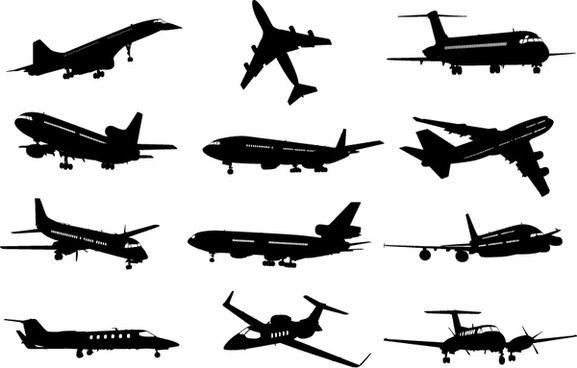
\includegraphics[width=1.1\textwidth]{cover}
\end{center}

\pagebreak

\tableofcontents
 
\pagebreak

\section{Introduction}

Sharks are a part of the chondricthyes family.

\subsection{A subsection}

More text.

\section{Airplanes}

Your text goes here.

\subsection{Wings}

More text.

\subsubsection{Flaps}

More text.

\subsection{Fuselage}

More text.

\section{Analysis}

Your text goes here.

\subsection{Balanced Field Length}

More text.

\subsection{PyTornado}

Link to PyTornado Documentation: 

\url{https://pytornado.readthedocs.io/en/latest/index.html}

\subsection{Range}

More text.

\subsection{Specific Excess Power}

More text.

\subsection{Trim}

More text.

\subsubsection{Linear Trims}

More text.

\section{Modeling}

Your text goes here.

\subsection{Aerodynamics}

More text.

\subsection{Propulsion}

More text.

\section{Common}

Your text goes here.

\subsection{Atmosphere}

More text.

\subsection{Earth}

More text.

\subsection{Equations of Motion}

More text.

\subsection{Rotations}

More text.

\end{document}
